\documentclass[12pt,a4paper]{report}

\usepackage{epcc}
\usepackage{graphics}
% \usepackage{mathtools}
\usepackage{amsmath}

% This example file shows how a thesis can be laid out using Latex. It
% does not use any special local features so should be portable to other
% places.
% 
% When producing draft copies of a thesis you may want to print only
% selected pages of the thesis. To do this use the command
% 
% dvips -f -p 4 -n 3 myfile.dvi | lpr
% 
% where -p 4 means start printing at page 4 (ie the page that will be
% numbered 4, not necessarily the 4th page) and -n 3 means print 3 pages.
% This example will print pages 4, 5 and 6.
% 
% If you want to print the thesis and also save paper you can print more
% than one page on each sheet of paper. Use the command
% 
% dvips -f myfile.dvi | psnup -2 | lpr
% 
% to print 2 pages per sheet. psnup can take values 2, 4, 8, or 9.
%
% To produce a PDF version you can create a PostScript copy first
%
% dvips -f myfile.dvi > myfile.pdf
%
% and then convert it
%
% distill myfile.ps
%
% or you can go straight to PDF
%
% pdflatex myfile
%
% Note that pdflatex expects all included figures to be in PDF too. See
% the includegraphics command below.


% This document contains many cross-references and forward references,
% eg in constructing a table of contents, so Latex may need to be run
% twice to get all the references correct. If you need to run Latex twice
% you may get the warning:
% 
% LaTeX Warning: Label(s) may have changed. Rerun to get cross-refSerences right.


% the following 4 lines are the content of the smallmargins.sty file
% but including them explicitly makes this more portable.
%AC%\oddsidemargin=0.1in
%AC%\topmargin=-0.5in
%AC%\textheight=9in
%AC%\textwidth=6.25in

%AC%\parskip 10pt
%AC%\parindent 0in

\begin{document}

%AC%\pagestyle{myheadings}
%AC%\markright{D.~S.~Henty}

%\title{A Latex thesis example}
%\author{D.~S.~Henty}
%\date{\today}

%\maketitle

\pagenumbering{roman}

\title{Bayesian Inference Using Sequential Monte-Carlo Algorithm for Dynamic System Models}
\author{Chaolin Han}
\date{\today}

\makeEPCCtitle

\thispagestyle{empty}

\vspace{11cm}

\begin{center}

\large{MSc in High Performance Computing}

\large{The University of Edinburgh}

\large{Year of Presentation: 2020}

\end{center}

\newpage

\begin{abstract}
This is the bit where you summarise what is in your thesis.
\end{abstract}

\pagenumbering{roman}

\tableofcontents
\listoftables
\listoffigures

\begin{titlepage}
\vspace*{2in}
% an acknowledgements section is completely optional but if you decide
% not to include it you should still include an empty {titlepage}
% environment as this initialises things like section and page numbering.
\section*{Acknowledgements}

This template is a slightly modified version of the one developed by
Prof. Charles Duncan for MSc students in the Dept. of Meteorology. His
acknowledgement follows:

{\em This template has been produced with help from many former students who
have shown different ways of doing things. Please make suggestions for
further improvements.}

\end{titlepage}

\pagenumbering{arabic}

\chapter{Introduction}
This should contain a description of your project and the problem you
are trying to solve. Where appropriate you should also include
references to work which has already been done on your topic and
anything else which lets you set your work in context.

One of the things you will need to do is to ensure that you have a
suitable list of references.  To do this you should see \cite{ref:lam}
or some other suitable reference.  Note the format of the citation used
here is the style favoured in this department.  Here is another
reference \cite{ref:bloggs} for good measure.

You will also want to make sure you have no spelling or grammatical
mistakes. To help idwentify spelling mistukes you caan use the commands
{\em ispell} or {\em spell}. See the appropriate manual pages. Remember
that spelling mistakes are not the only errors which can occur. Spelling
checkers will not find errors which are, in fact, valid words such as
{\em there} for {\em their}, nor will they find repeated words which
sometimes occur if your concentration is broken when typing. {\bf There
is no substitute for thorough proof reading!}


[background and motivation]

[what is done]

\chapter{Background}

\section{Zebrafish spinal cord regeneration}

[describe the process and how cells and cytokines are involved]

\section{Mathematical modelling}

[how this can be modelled as dynamic systems]

[general topics of mathematical models: how to build model according to interactions; how to calibrate/ parameterise the model; how to solve the model; dynamics; how to evaluate the model]
 

\section{Bayesian inference}

[how to parameterise the model]

[how the infer the parameter given data]

[likelihood-free inference and information about ABC SMC]

[model comparison, ABC SMC for model comparison]

\section{Software tools}

[existing tools and software for this task]

[workflow and developing]

\chapter{Mathematical modelling}

Mathematical models can describe different kinds of dynamic system, and can be used as a guide to prediction and analysis. An ideal model in this case, can represent reasonable interactions/effects between cells and cytokines and recover the observed  trend against time. 

Models for the regeneration process is in the form of ordinary differential equations, specifically the time differential form. Terms in the ODE are mostly explainable and corresponds interaction paths. 

\section{Observed data}

Our models is built regarding the existing experiments data form Tsarouchas et al.\cite{ref:Tsarouchas}. The measurement includes the number of three kinds of cells (neutrophil $N$, macrophage $\Phi$ and microglia) and the relative concentration of four cytokines (il-1$\beta$, tnf-$\alpha$, tgf-$\beta$1a and tgf-$\beta$3). As proposed in \cite{ref:Tsarouchas}, neutrophil and macrophage play important roles in the promotion of spinal cord regeneration with il-1$\beta$ and tnf-$\alpha$ being the mediation. According to this, our current models focus on the changes of four variables $N$, $\Phi $, $\beta$ (il-1$\beta$) and $\alpha$ (tnf-$\alpha$). $N$ and $\Phi$ is of the unit `number of cells', $\beta$ and $\alpha$ is of the unit `relative concentration'.

It is noted that the variance of the measured data is relatively high. The summary statistic used for the parameter estimations is mean of measurement, assuming that measured data is Gaussian-like distributed. The distribution of the measured data points is plotted and examined to see if the measurement mean could represent the distribution. The result is that at most time points the measurement values are Gaussian-distributed, some distributions are skewed. One abnormal distribution is observed at time point 120 h post-lesion (hpl) for macrophage where there are two concentrations. Mean value can summarise most data measures and thus is still used as the target summarised observed data. A plot of the mean of the four variables is shown in Figure \ref{fig:obs_data}

\begin{figure}
\begin{center}
\resizebox{1.0\hsize}{!}{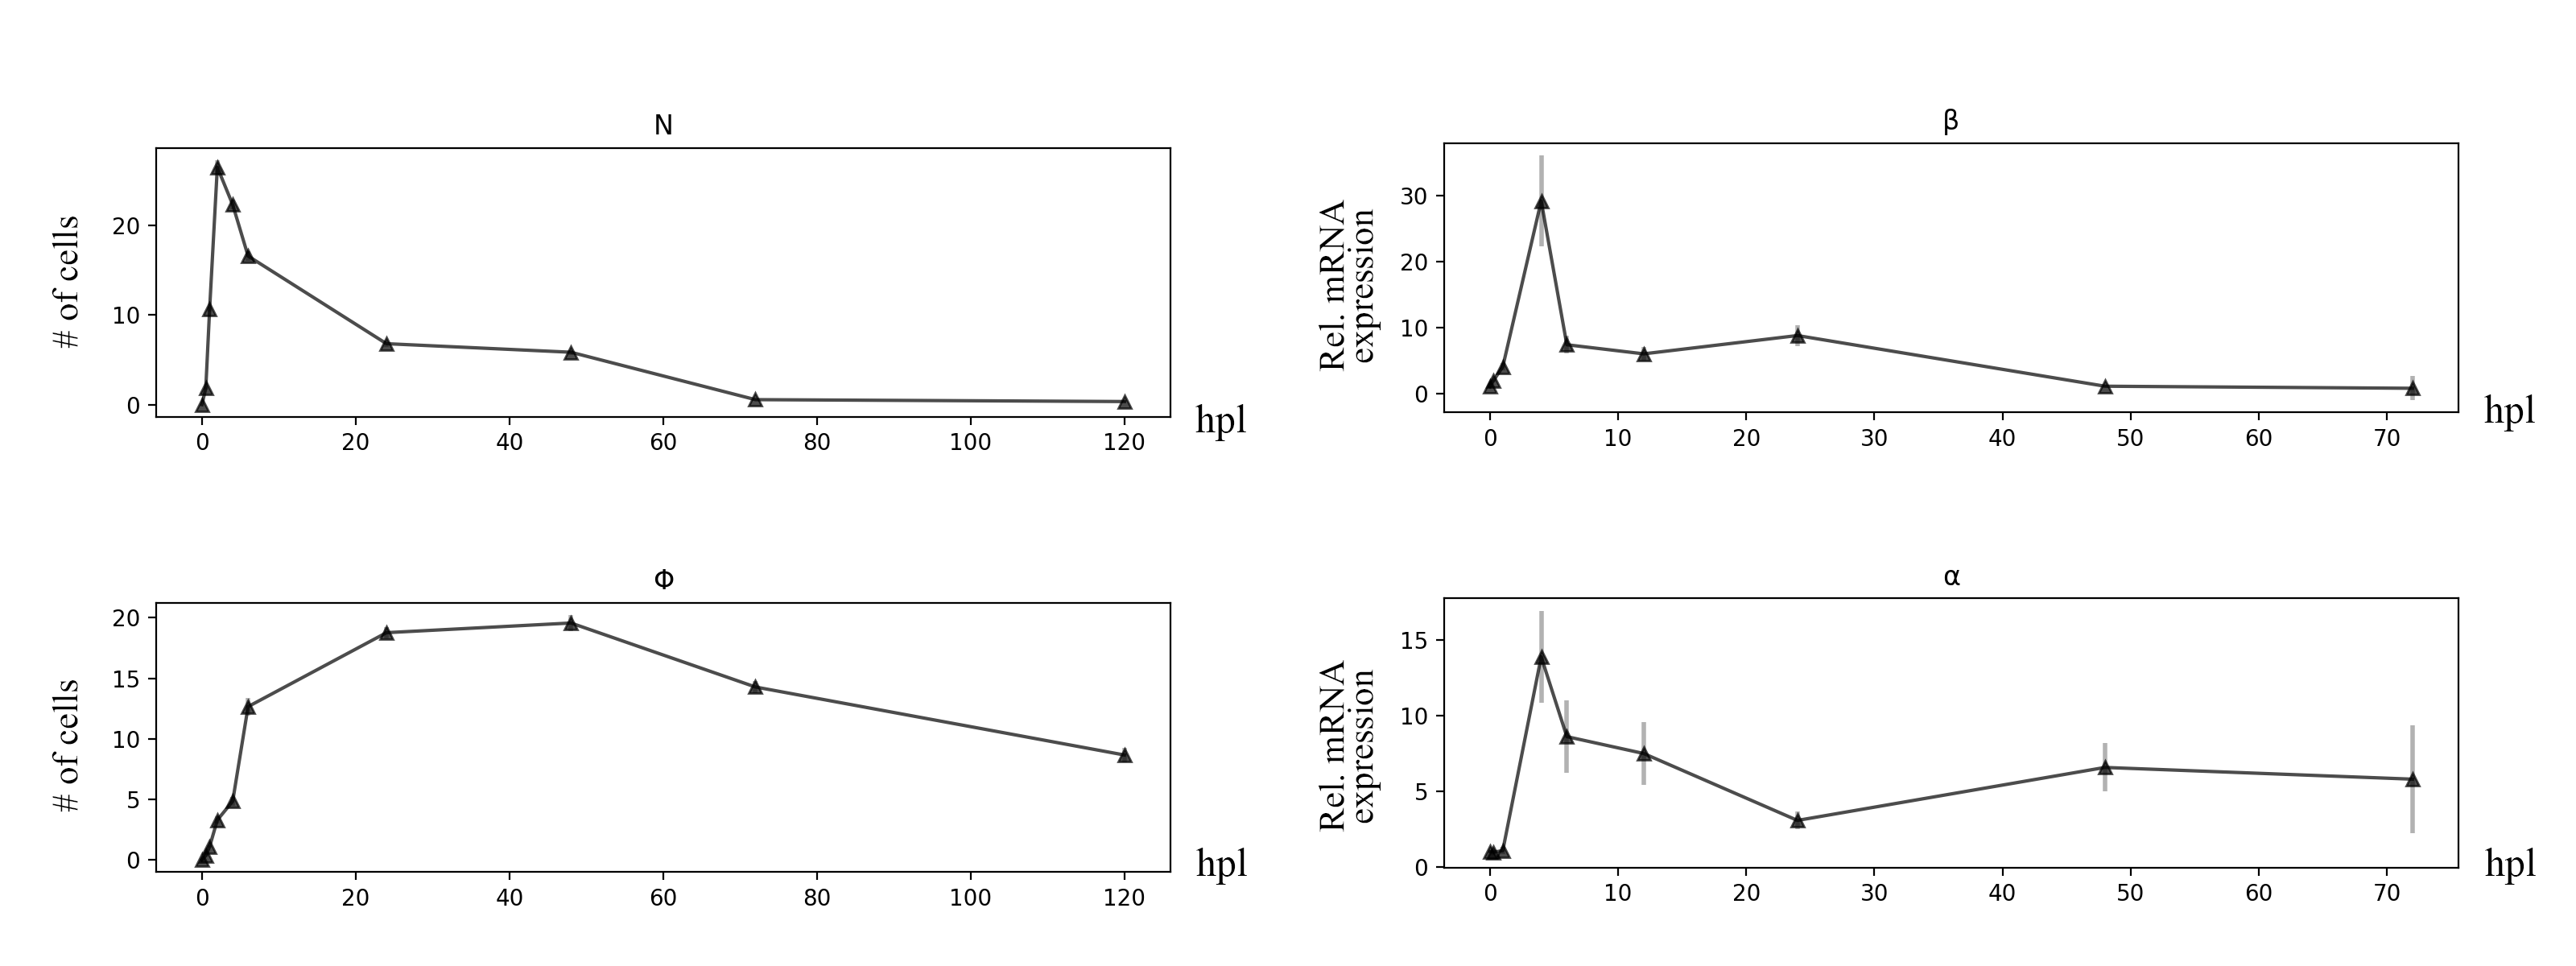
\includegraphics{fig/obs_curve.png}}
\end{center}

\caption[Mean of the observed data]%
{Mean of the observed data for neutrophil $N$, macrophage $\Phi$, il-1$\beta$ and tnf-$\alpha$, from experiment results of \cite{ref:Tsarouchas}. Error bars indicate standard error of mean} 
\label{fig:obs_data}

\end{figure}

\section{Hypothesis and Models}

5 models in total are proposed according to different hypothesis. At first our tests and implementations of ABC SMC for parameter estimations use only the basic model for developing propose. After the parameter estimation framework is built and tested, more models are proposed, in order to calibrate and adjust the basic model such that it can be more close to the true process, recover more features of the observed data or test our hypothesis. 

All these models assumes the interactions is within two kinds of cells (neutrophil and macrophage) and two kinds of cytokines (il-1$\beta$ and tnf-$\alpha$) and use the data presented in Figure \ref{fig:obs_data} for parameter estimation. Interactions or effects from other cells or cytokines is not considered as there might not be corresponding data.

\subsection{Basic model}

A preliminary model is proposed according to \cite{ref:Tsarouchas} and used to build and test the code. A interaction map illustrate the model is shown in Figure \ref{fig:m1}. This model is a simplification a the process described in \cite{ref:Tsarouchas}. To describe the parameters' units, we denote the unit of $N$ and $\Phi$ i.e. number of cells as `cell', and denote the unit of $\beta$ and $\aleph$ i.e. relative mRNA expression as `unit' for simplicity.

\begin{figure}
    \begin{center}
    \resizebox{0.4\hsize}{!}{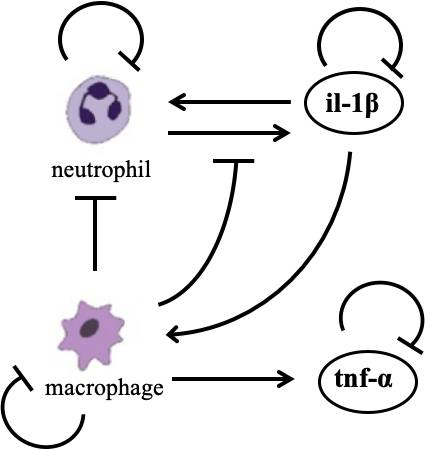
\includegraphics{fig/model1.png}}
    \end{center}
    
    \caption[Interactions modelled in the basic model]%
    {Interactions modelled in the basic model (model 1) based on Tsarouchas et al.\cite{ref:Tsarouchas}. Lines ended with arrow represent promoting effect, lines ended with T-connectors represent inhibition} 
    \label{fig:m1}
    
\end{figure}

It is assumed that there are negative feedbacks for all the variables. MORE DESCRIBE.

\begin{align}
    \label{eq:model1}
    \begin{split}
        &\frac{\mathrm{d} N}{\mathrm{d} t}=\lambda_N+\kappa_{N\beta}\beta-\mu_NN-\nu_{N\Phi}N\Phi\\
        &\frac{\mathrm{d} \Phi}{\mathrm{d} t}=\lambda_\Phi+\kappa_{\Phi\beta}\beta-\mu_\Phi\Phi\\
        &\frac{\mathrm{d} \beta}{\mathrm{d} t}=\frac{s_{\beta N}N}{1+i_{\beta\Phi}\Phi}-\mu_\beta\beta\\
        &\frac{\mathrm{d} \alpha}{\mathrm{d} t}=s_{\alpha\Phi}\Phi-\mu_\alpha\alpha
    \end{split}
\end{align}

\begin{table}[h!]
\centering
\begin{tabular}{|c c c|} 
 \hline
 Parameter & Definition & Units\\ [0.5ex] 
 \hline\hline
 $\lambda_N$ & Self-increase rate of neutrophil & $cell/h$  \\ 
 $\kappa_{N\beta}$ & Promoting effect coefficient by il-1$\beta$ & $cell/(unit\cdotp h)$\\
 $\mu_N$ & Coefficient of negative feedback of $N$ & $h^{-1}$ \\
 $\nu_{N\Phi}$ & Coefficient of inhibition of both $N$ and $\Phi$& $cell^{-1}\cdotp h^{-1}$ \\
 \hline
 $\lambda_\Phi$ & Self-increase rate of macrophage & $cell/h$ \\
 $\kappa_{\Phi\beta}$ & Promoting effect coefficient by il-1$\beta$ & $cell/(unit\cdotp h)$ \\
 $\mu_\Phi$ &  Coefficient of negative feedback of $\Phi$ & $h^{-1}$ \\
 \hline
 $s_{\beta N}$ & Production rate from $N$ & $unit/(cell\cdotp h)$ \\
 $i_{\beta\Phi}$ & Coefficient of inhibition to the production & $cell^{-1}$ \\
 $\mu_\beta$ & Coefficient of negative feedback of $\beta$ & $h^{-1}$ \\
 \hline
 $s_{\alpha\Phi}$ & Production rate from $\Phi$ & $unit/(cell\cdotp h)$ \\
 $\mu_\alpha$ & Coefficient of negative feedback of $\alpha$ & $h^{-1}$ \\
[1ex] 
 \hline
\end{tabular}
\caption{Parameters introduced in the basic model (model 1)}
\label{table:m1}
\end{table}

\subsection{Alternative models}

\paragraph{Model 2 and model 3}

As the observed data indicates, this dynamic system has a steady state where the  inflammation is resolved and immune cells should not be present at the injury site. Regarding this, the self-increase term $\lambda$ cannot be constant, thus a exponentially decay $\lambda$ term is introduced and model 2 is proposed as Eqn. \ref{eq:model2}. The inhibition of il-1$\beta$ being produced by neutrophil, i.e. $i_{\beta\Phi}$ is considered to be ignored, in which case the relative expression of il-1$\beta$ is only affected by the number of neutrophil and the negative feedback from itself. This case corresponds to model 3, written as Eqn. \ref{eq:model3}.

Model 2 and model 3 has one extra parameter $a$ which is a coefficient in the exponentially decay determining the decay speed, with the unit $h^{-1}$.

\begin{align}
    \label{eq:model2}
    \begin{split}
        &\frac{\mathrm{d} N}{\mathrm{d} t}=\lambda_Ne^{-at}+\kappa_{N\beta}\beta-\mu_NN-\nu_{N\Phi}N\Phi\\
        &\frac{\mathrm{d} \Phi}{\mathrm{d} t}=\kappa_{\Phi\beta}\beta-\mu_\Phi\Phi\\
        &\frac{\mathrm{d} \beta}{\mathrm{d} t}=\frac{s_{\beta N}N}{1+i_{\beta\Phi}\Phi}-\mu_\beta\beta\\
        &\frac{\mathrm{d} \alpha}{\mathrm{d} t}=s_{\alpha\Phi}\Phi-\mu_\alpha\alpha
    \end{split}
\end{align}

\begin{align}
    \label{eq:model3}
    \begin{split}
        &\frac{\mathrm{d} N}{\mathrm{d} t}=\lambda_Ne^{-at}+\kappa_{N\beta}\beta-\mu_NN-\nu_{N\Phi}N\Phi\\
        &\frac{\mathrm{d} \Phi}{\mathrm{d} t}=\kappa_{\Phi\beta}\beta-\mu_\Phi\Phi\\
        &\frac{\mathrm{d} \beta}{\mathrm{d} t}=s_{\beta N}N-\mu_\beta\beta\\
        &\frac{\mathrm{d} \alpha}{\mathrm{d} t}=s_{\alpha\Phi}\Phi-\mu_\alpha\alpha
    \end{split}
\end{align}

Model 3 can be regarded as a simplification of model 2, as it can be regarded as model 2 with parameter $i_{\beta\Phi}=0$. For these three models, model 1 is a naive one that is proposed at very first time and used as a `template' to build and test parameter inference framework. As the implementation is successful, model 2 and 3 is proposed. After fitting model 2 is supposed to be better than model 1 as it corrects the problem that appears at the final time points which are close to steady states for neutrophil and macrophage. model 3 is a small simplification of model 2 and theoretically less general than model 2.

\paragraph{Model 4 and model 5}

After the first model selection experiment, it is found that some significant features presented in the observed data is not recovered by any of the model. According to that, attempts are tried to introduce more interactions within the dynamic system considering the both biological and  mathematical context. Extra promoting effect to the expression of tnf-$\alpha$ is considered, by either add a phenomenological term (which means the same effect as directly promoting but the underlying mechanism is unclean) or add a term that represents a promoting effect to the production process of tnf-$\alpha$, namely model 4 (Eqn. \ref{eq:model4}) and model 5 (Eqn. \ref{eq:model5}).

\begin{align}
    \label{eq:model4}
    \begin{split}
        &\frac{\mathrm{d} N}{\mathrm{d} t}=\lambda_Ne^{-at}+\kappa_{N\beta}\beta-\mu_NN-\nu_{N\Phi}N\Phi\\
        &\frac{\mathrm{d} \Phi}{\mathrm{d} t}=\kappa_{\Phi\beta}\beta-\mu_\Phi\Phi\\
        &\frac{\mathrm{d} \beta}{\mathrm{d} t}=s_{\beta N}N-\mu_\beta\beta\\
        &\frac{\mathrm{d} \alpha}{\mathrm{d} t}=s_{\alpha\Phi}\Phi-\mu_\alpha\alpha+d_{\beta\alpha}\beta
    \end{split}
\end{align}

\begin{align}
    \label{eq:model5}
    \begin{split}
        &\frac{\mathrm{d} N}{\mathrm{d} t}=\lambda_Ne^{-at}+\kappa_{N\beta}\beta-\mu_NN-\nu_{N\Phi}N\Phi\\
        &\frac{\mathrm{d} \Phi}{\mathrm{d} t}=\kappa_{\Phi\beta}\beta-\mu_\Phi\Phi\\
        &\frac{\mathrm{d} \beta}{\mathrm{d} t}=s_{\beta N}N-\mu_\beta\beta\\
        &\frac{\mathrm{d} \alpha}{\mathrm{d} t}=(s_{\alpha\Phi}+f_{\beta\alpha}\beta)\Phi-\mu_\alpha\alpha
    \end{split}
\end{align}

\begin{table}[h!]
    \centering
    \begin{tabular}{|c c c|} 
     \hline
     Parameter & Definition & Units\\ [0.5ex] 
     \hline\hline
     $d_{\beta\alpha}$ & Coefficient of promoting effect from $\beta$ & $h^{-1}$  \\ 
     \hline
     $f_{\beta\alpha}$ & Coefficient of promoting the production of $\alpha$ by $\beta$ & $cell^{-1}\cdotp h^{-1}$  \\ 
    [1ex] 
     \hline
    \end{tabular}
    \caption{Parameters introduced in model 4 and 5}
    \label{table:m45}
\end{table}



\subsection{Model evaluation and comparison}

[feasible or not; goodness of fit; features of these models]

[bayes factor for model selection]

\subsection{Limitations}

[hypothesis]

[available data]

[model misspecification]

% \begin{figure}

% \begin{center}
% \resizebox{0.30\hsize}{!}{
\includegraphics{logos/crest_bw}}
% \end{center}

% \caption{The University Crest}
% \label{fig:eucrest}

% \end{figure}


% see the man page for dvips for details of the special command which is
% much more powerful than is shown here. It allows offsets in the
% horizontal and vertical and scaling in x and y.

% choosing suitable values for offset and scale can be a tiring matter
% of trial and error.

% note that labels do not need to include a description of the object
% they are labelling but it can be helpful, eg \label{fig:figurename}.

% You can use a label on a figure to refer to it later. The university
% crest is in \ref{fig:eucrest}. Note that you should not use phrases like
% ``the figure above'' or ``the following figure'' since Latex may move
% the figure relative to the text if it cannot be fitted onto the current page.

\chapter{Implementations and Experiments}

This chapter focuses on the implementation of the ABC SMC on the proposed models. Estimation of  parameters in the proposed models is the main task of this section. ABC SMC-based models selection is another task that can be easily implemented with the parameter estimation framework.

The build and test is under \verb|Python| environment with \verb|pyABC|\cite{ref:pyabc}. Some other code e.g. shell script and \verb|R| code are also used to perform the experiments and analyse the results. Tested software and system environment can be found at Appendix A. The build and test is performed on local computers and HPC clusters available within EPCC.

\section{Parameter estimation}

[implementation details and options/ settings that are affecting the ABC]

As the key focus of this project is on the parameter estimations of dynamical system, the ability of inference on the proposed model is firstly examined before actual inference using the experimental observed data.

In the first part, synthetic data is used with known true parameter values. The algorithm implementation is evaluated by the efficiency and goodness of resultant model under different implementation options and ABC SMC hyperparameters.

Then according to findings in the first part, several options with good performance are tried in the inference using experimental observed data (Figure \ref{fig:obs_data}). To obtain a more accurate and general results, these experiments are repeated for 3 or more times.

\subsection{ABC SMC and model hyperparameters experiments}

[including the options that are tested/ tried/ not adopted]

[including experiments results and discussions]

[how do these options correspond to biological model and how to set them accordingly for proposed model]

The ABC SMC inference can have largely different performance when using different hyperparameters and implementation options. To firstly test the ability of inference and observe the results of different options, synthetic data with known true parameter values are used as target data. The true value of parameters that are used to generate synthetic data is listed in Appendix B.1. These true values are firstly obtained by fitting a least square fit of model 1 onto the experimental data (Figure \ref{fig:infer_back_data}), the target data is then generated using these parameter values via ODE solver in \verb|Python|.

\begin{figure}
    \begin{center}
    \resizebox{1.0\hsize}{!}{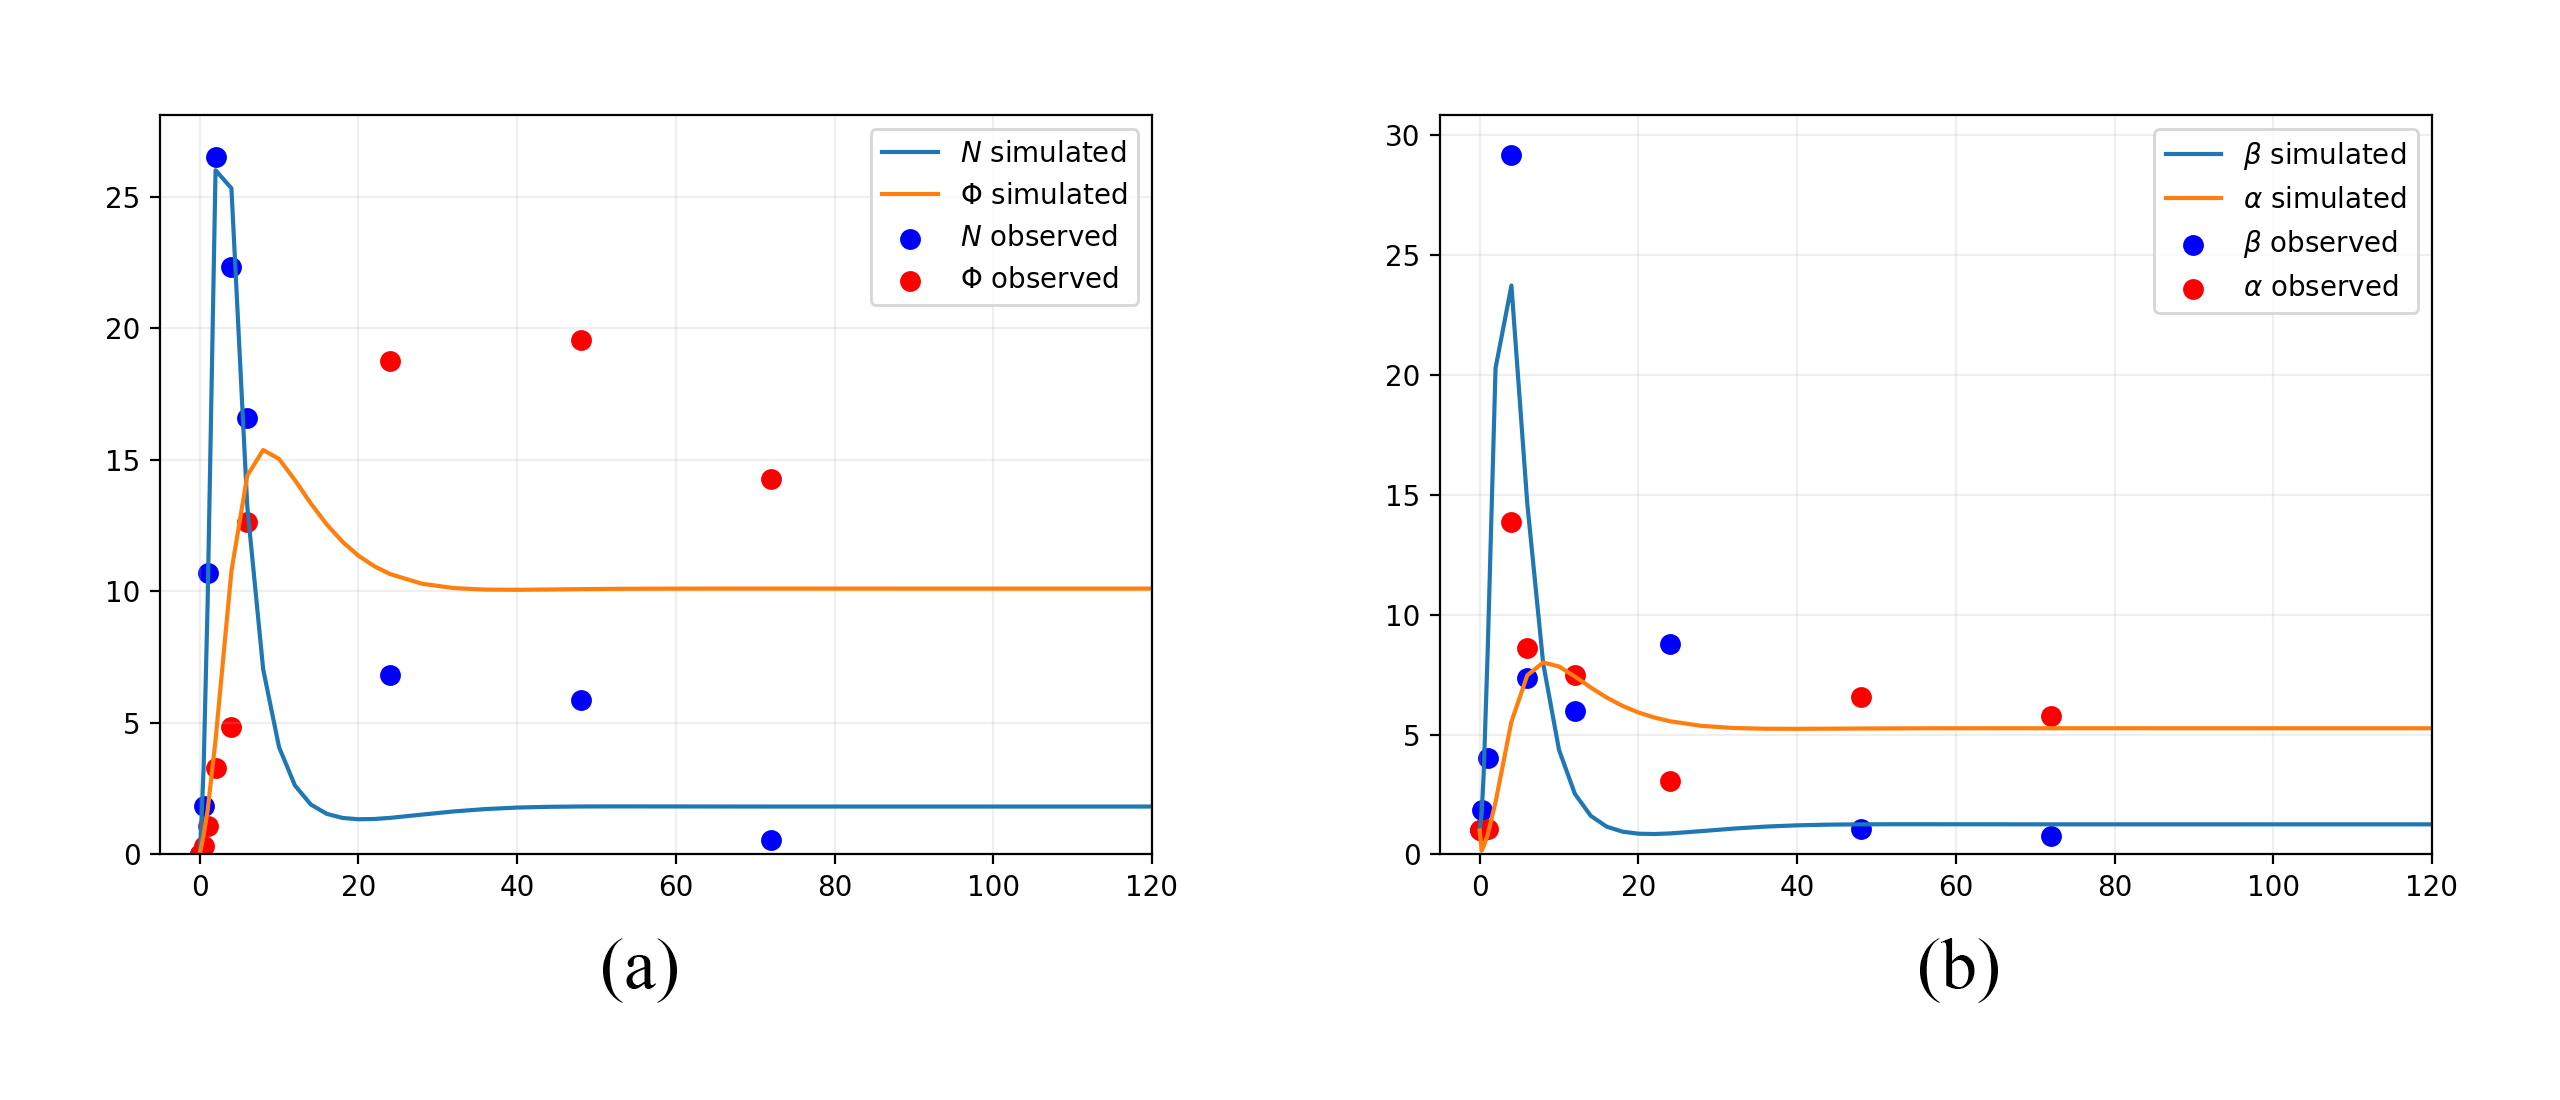
\includegraphics{fig/LS.png}}
    \end{center}
    
    \caption[Synthetic data generated with known parameter values]%
    {Synthetic data generated with known parameter values (line plot), compared to experimental data (scatter plot)} 
    \label{fig:infer_back_data}
    
\end{figure}

Among them the following topics are studied using synthetic data.

\subsubsection{Perturbation kernels}

Perturbation kernels work in the sampling process. In each generation $t$, samples are firstly taken from the previous population $\{\theta_{t-1}\}$ with weights $\{w_{t-1}\}$, then perturbed using the perturbation kernel $K(\theta|\theta^*)$. We keep sampling until $N$ particles are accepted, where $N$ is the pre-set population size. After that the new weights are calculated and normalised. 

\begin{figure}
    \begin{center}
    \resizebox{1.0\hsize}{!}{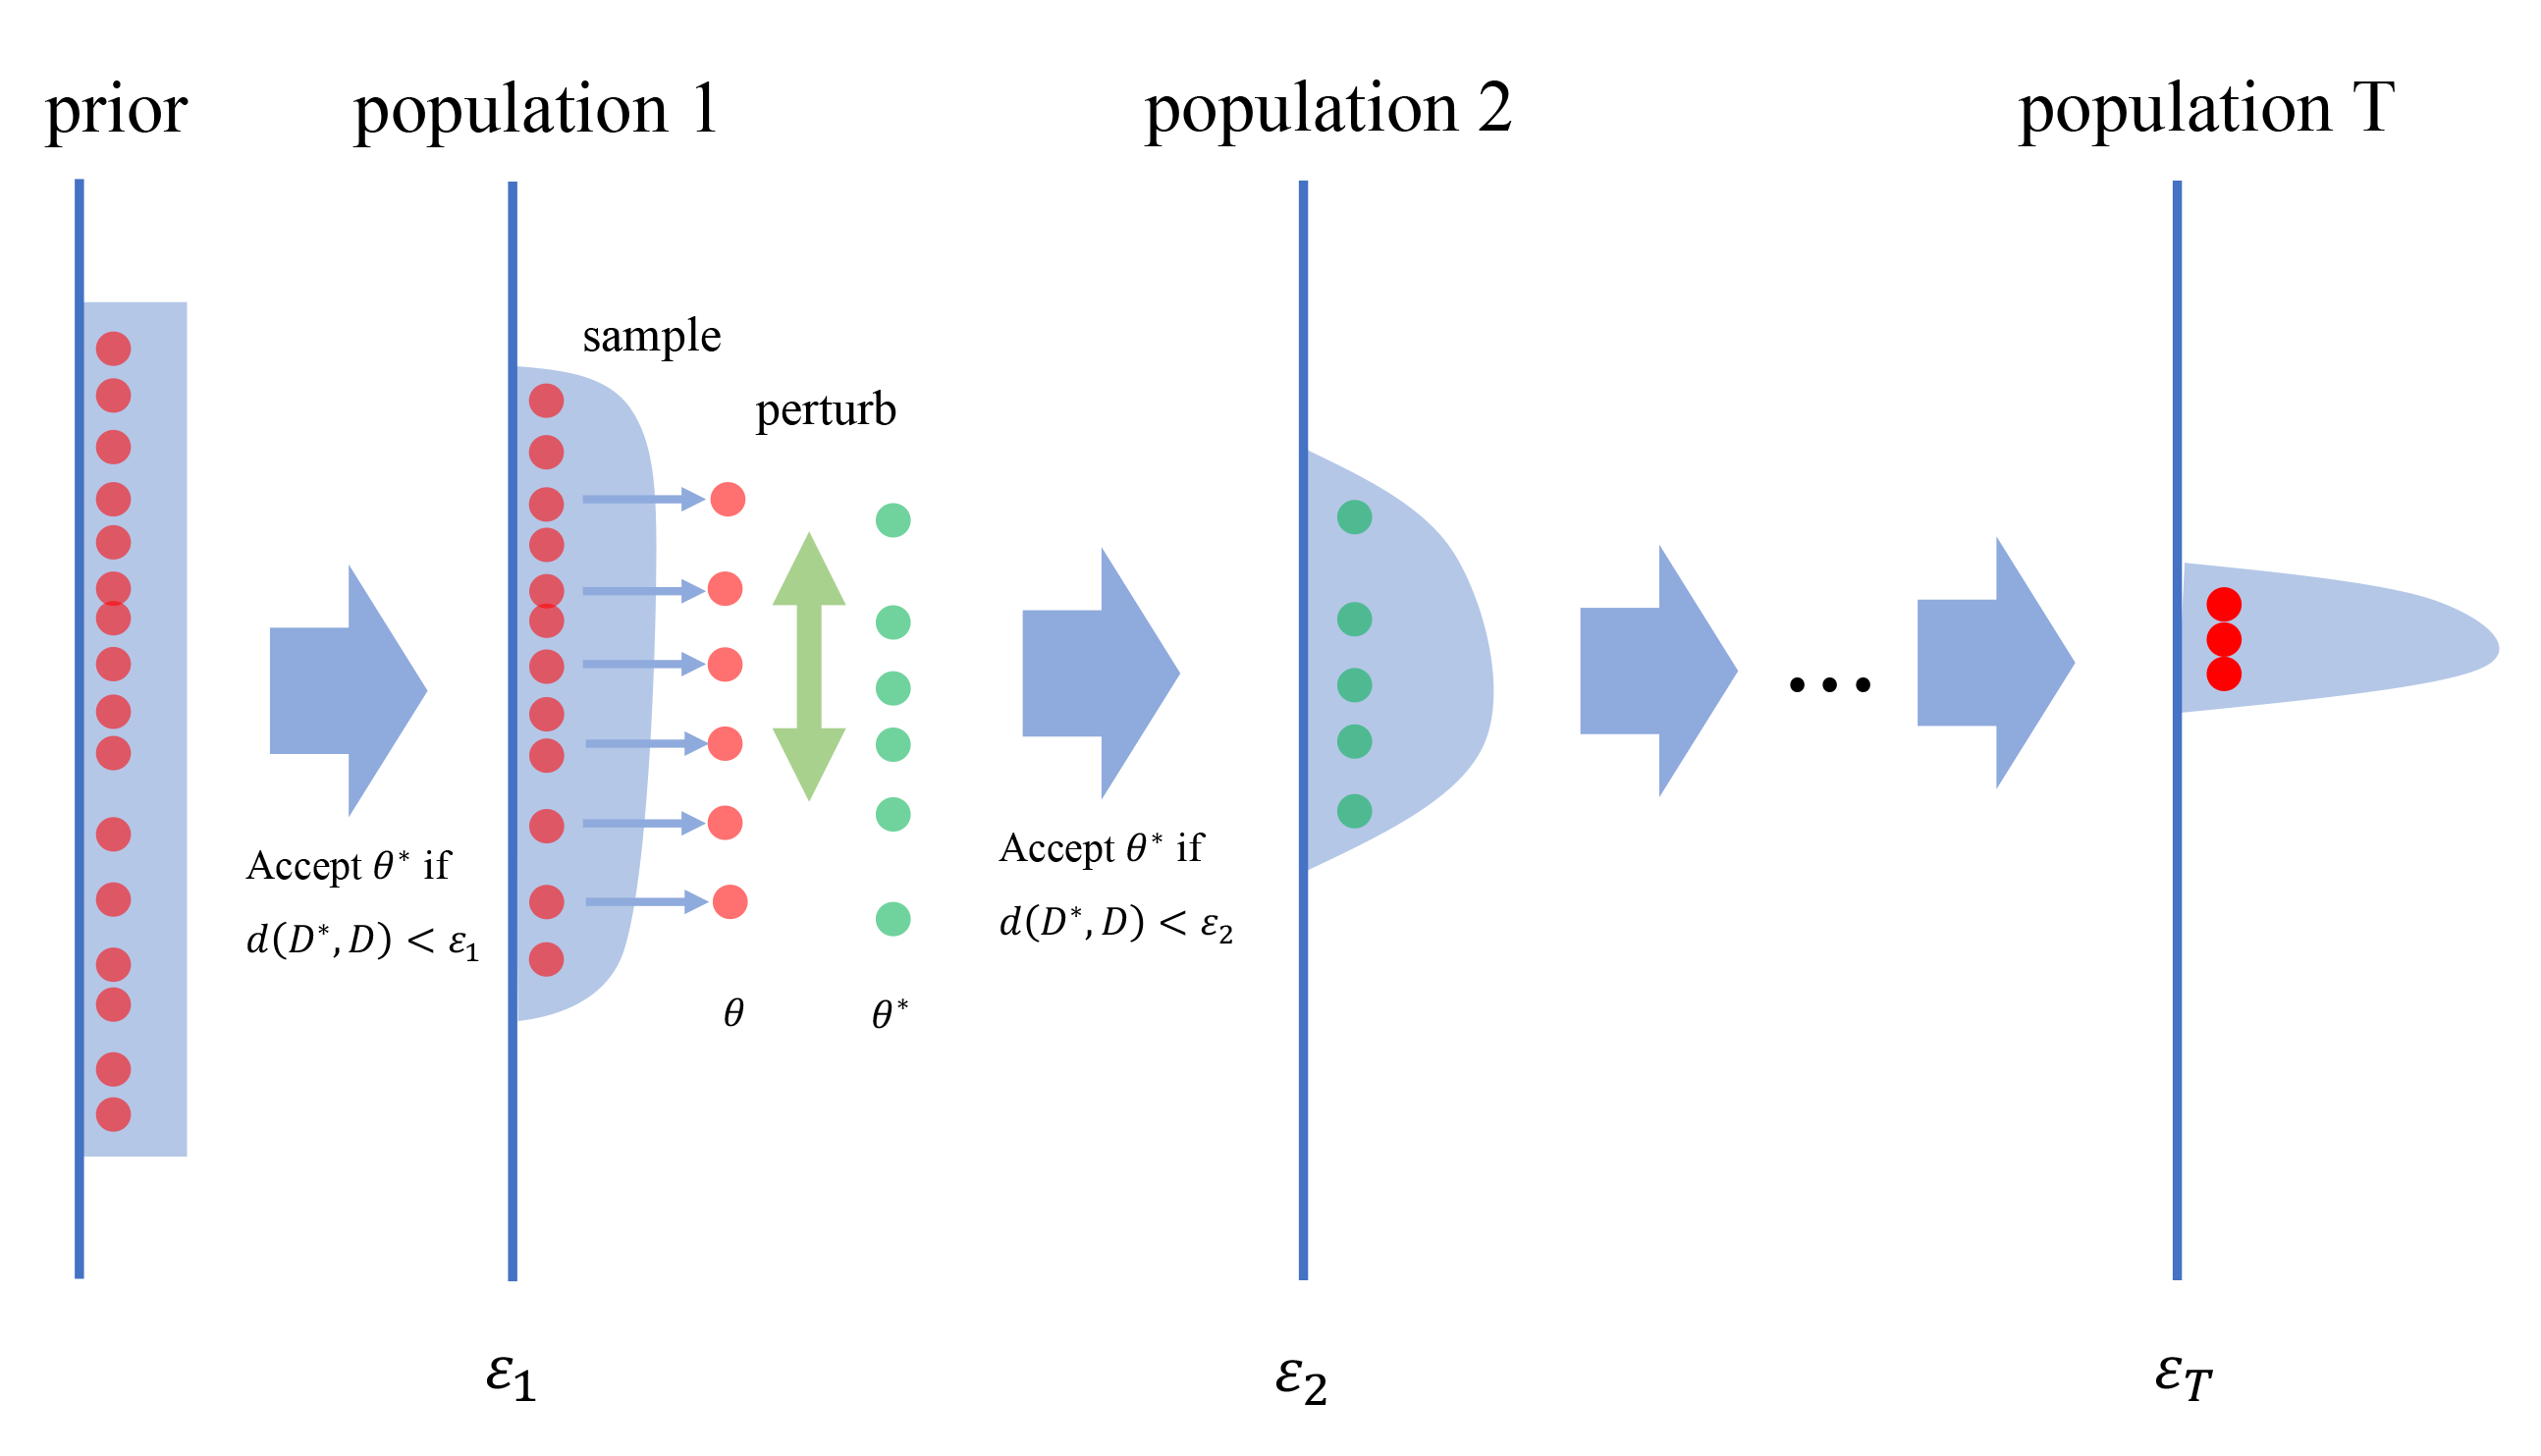
\includegraphics{fig/smc.png}}
    \end{center}
    
    \caption{ABC SMC sampling process} 
    \label{fig:smc}
    
\end{figure}

The perturbation kernel is called in the sampling of every particles and determines how the new perturbed particle is chosen, thus it is influential to both computation complexity and the resultant posterior distribution. Generally, a local perturbation kernel may face the risk of being stuck in local modes (e,g., local optimal), but it may need less computational operations, or could generate a population with a higher acceptance rate if the successive epsilon values are close; A kernel with wide variance, or spreading out in a large space could help in resolving the local optimal problem by a more thoroughly exploration of the parameter space, however it can be more computation-intensive and result in a lower acceptance rate. A desired optimal kernel should balance the trade-offs; their property and criteria is discussed in \cite{ref:kernel}.

There are several common choice of perturbation kernels. Among them multivariate normal kernel and local M-nearest neighbour model is preferred to be applied on our models. A covariance matrix $\Sigma_t$ of accepted particles is calculated form previous generation and used in multivariate normal kernel: $K(\theta|\theta_{t-1})\sim\mathcal{N}(\theta_{t-1}, \Sigma_t)$. It is illustrated to be more efficient than uniform kernel and component-wise normal kernel in relecting the true posterior structure \cite{ref:kernel}. It has been proved to perform well in several dynamic system models \cite{ref:abcsysbio, ref:compare, ref:disease} for the parameter estimation and model selection tasks. The $scaling\in(0,1]$ parameter in \verb|pyABC| will be multiplied to the covariance to produce a `narrower distributed' perturbation result.

Local M-NN kernel provided by \verb|pyABC| is also tried to provide a comparison. A local kernel density estimation (KDE) fit is used with M nearest neighbours considered.

The kernel experiments is designed to explore the efficiency of SMC on our dynamical systems. Given the same fixed threshold schedule, kernels that need less total samples and have higher acceptance rate would be our preference. The experiments compared multivariate normal kernel with local MNN kernels with different parameters, using synthetic data to infer back the parameters. The acceptance rate among each time point and total required samples are compared after the experiment to give suggestions on the kernel selection in the real data inference. As the threshold schedule is fixed, the final population should have similar discrepancy to the target data thus here the goodness of fit i.e. recover of target data trends/features and errors of the inferred parameters compared to true values is not discussed.

\subsubsection{Kernel experiment results}

To compare kernels, a fixed schedule schedule is used with minimal epsilon i.e. $\epsilon_t$ set to 10.0. From the total required samples graph Figure \ref{fig:kernel1}, the efficiency can be compared. Among the tested kernels, the local M-NN with M=50 has the best performance: it requires the least number of samples and 
has higher acceptance rates among almost all generations. Local M-NN with M=750 is the slowest kernel.

For local M-NN kernels, generally a greater M will lead to lower acceptance rate and 
more required particles in each generation. As shown in Figure \ref{fig:acceptance1}, local M-NN with M=750 is the lowest curve. Consequently, if greater M is test, then it will have even lower acceptance rates; the maximum M=2000 (whole population is considered) will have the lowest acceptance rates.

\begin{figure}
    \begin{center}
    \resizebox{1.0\hsize}{!}{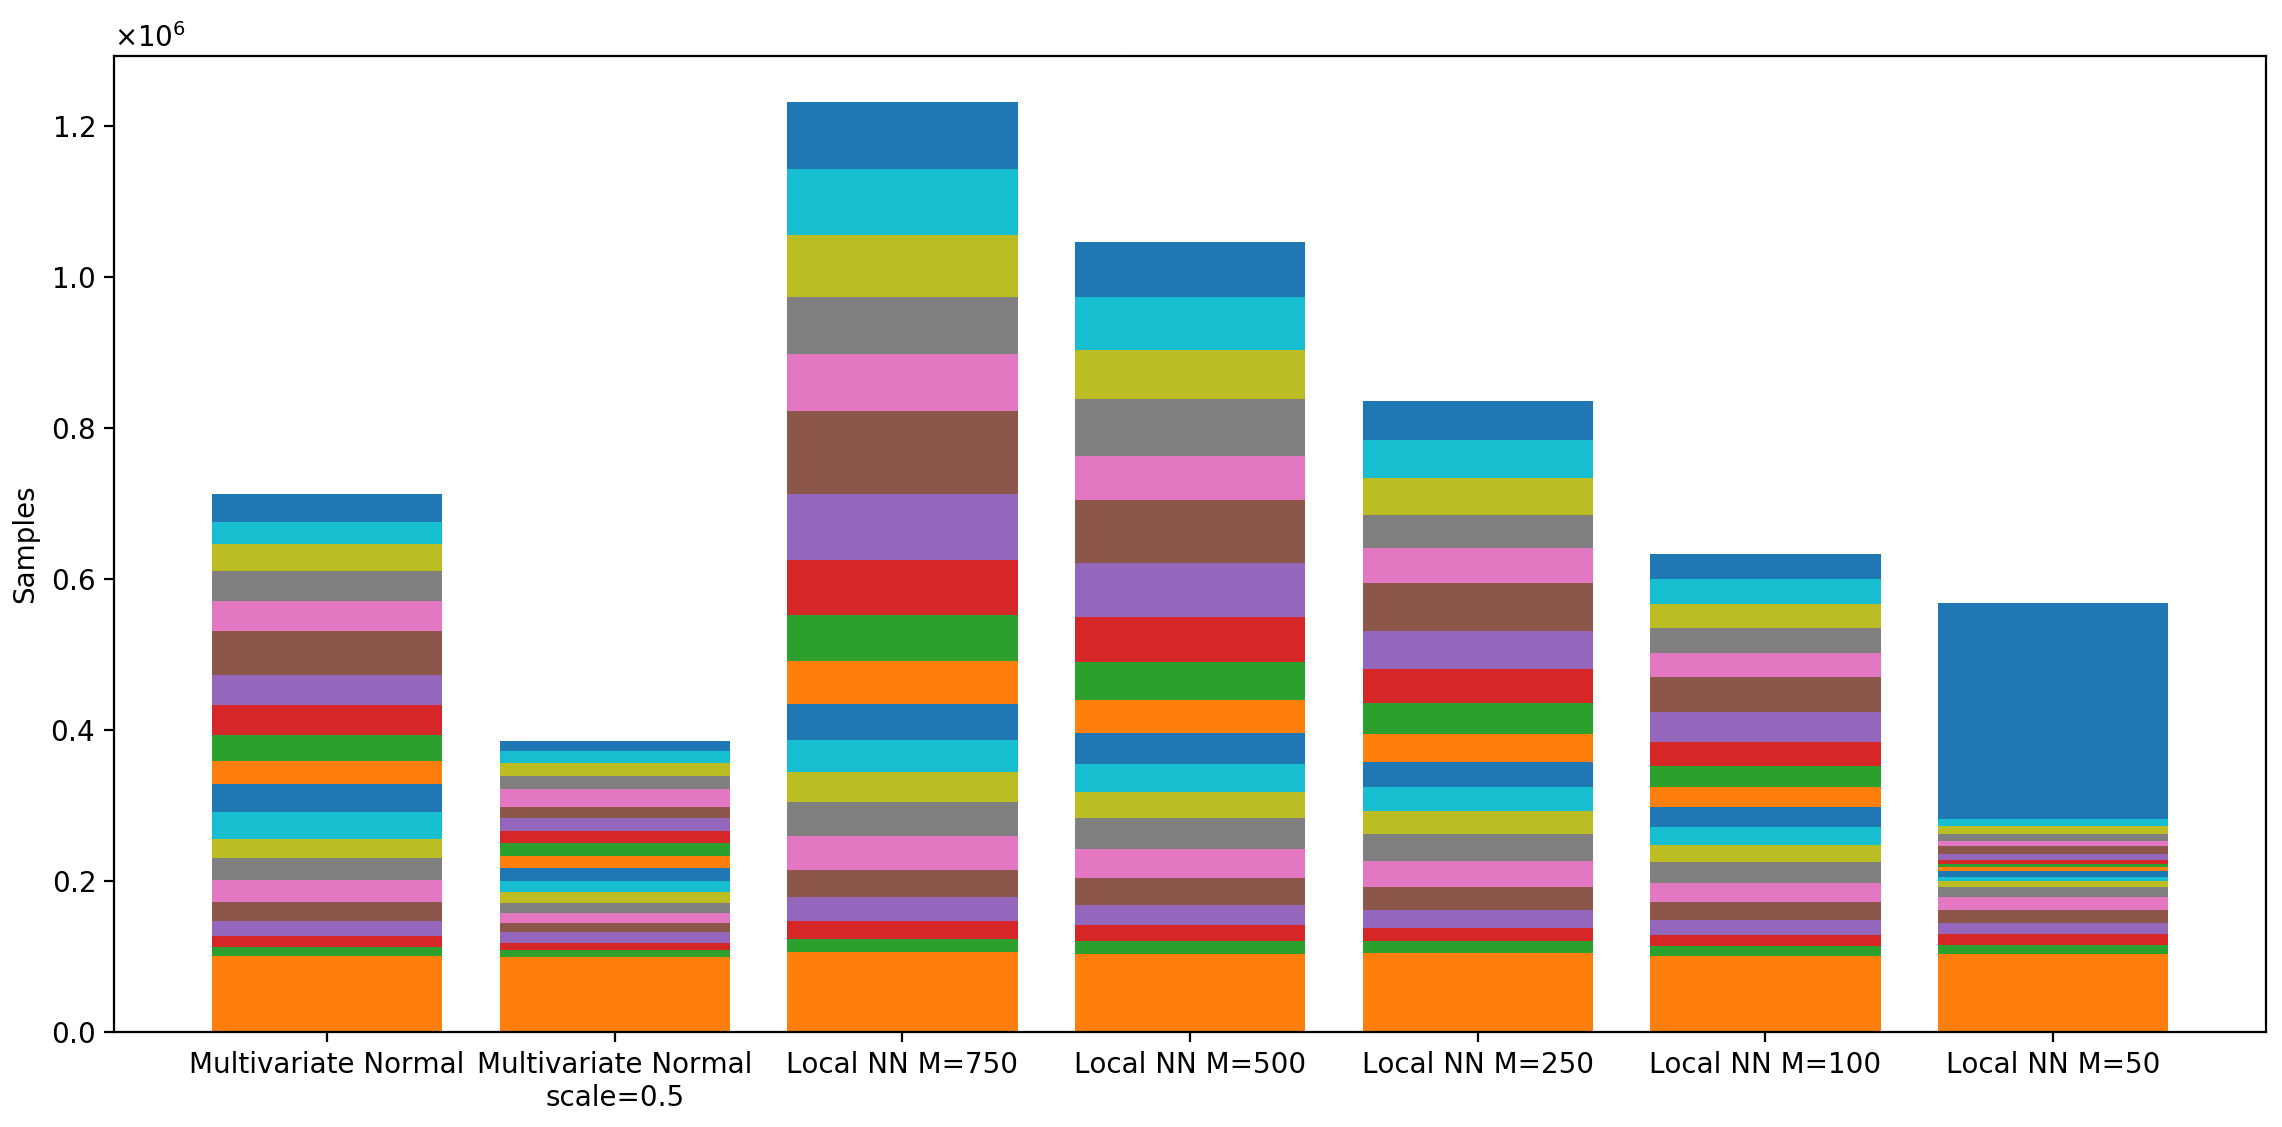
\includegraphics{fig/kernel1.png}}
    \end{center}
    
    \caption[Total required samples of different kernels]%
        {Total required samples of different kernels. Different color represents different generations (bottom to top: generation 1 to generation 20)}
    \label{fig:kernel1}

    \vspace*{\floatsep}

    \begin{center}
    \resizebox{1.0\hsize}{!}{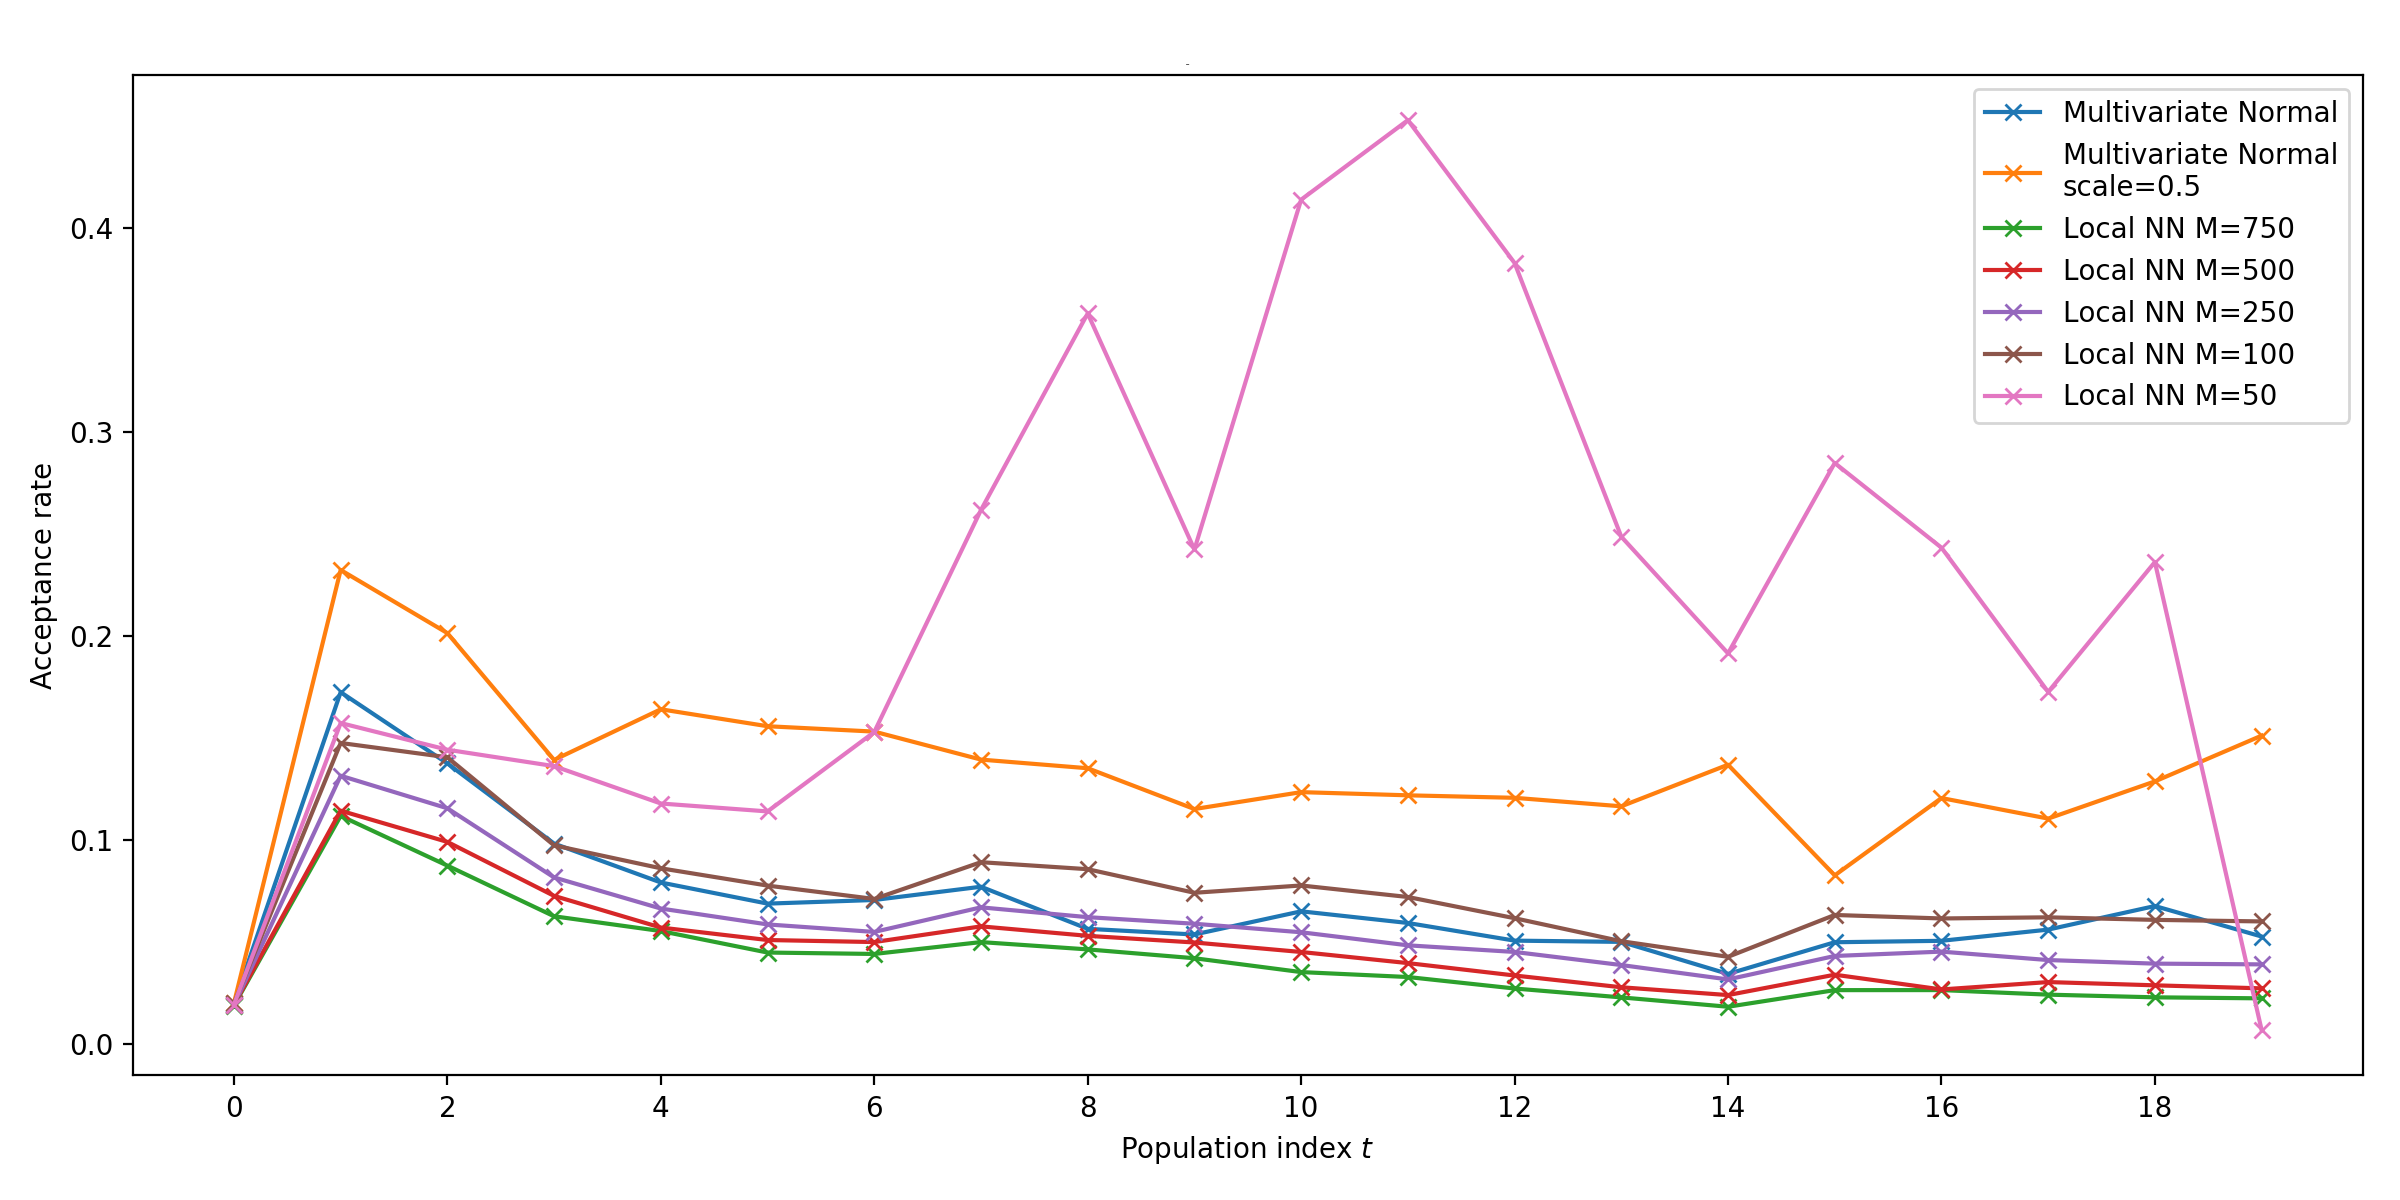
\includegraphics{fig/acceptance1.png}}
    \end{center}
    
    \caption{Acceptance rates of different kernels}
    \label{fig:acceptance1}
    
\end{figure}

Multivariate normal kernel has a performance between local M-NN M=250 and M=100. It proves that rather than a trivial normal kernel, multivariate normal kernels is more efficient facing the concentrations of joint distributions among multiple parameters \cite{ref:kernel}. `Scaling' option can narrower the distribution calculated from the last population, thus making the kernel more `local' by sampling under a smaller variance. Similar to small M in local M-NN, small `scaling' is also more efficient in our experiment of the model 1. Besides the fixed threshold schedule, a median threshold schedule with the same final threshold $\epsilon_{20}=10.0$ is also tested and similar results are observed (Figure \ref{fig:kernel2} and \ref{fig:acceptance2}, Appendix B2).

It seems that a more `local' kernel can give better performance by efficiently sampling around concentrations in parameters' distribution and approximate the posterior distribution. This holds in most cases under a given target final threshold value $\epsilon_t$, however may not produce the proper result want: a more local kernel, e.g. local M-NN with small M and multivariate normal with `scaling' is more likely to be stuck in local optimality, as the kernel is less likely to sample particles that are far from local concentrations, although these local optimal are still accepted under given threshold. In other words, using local kernels the epsilon may quickly converge to to local optimal; if a even smaller epsilon is desired, the local kernel can hardly generate enough particles to find another matched local modes. Also, the shapes of posterior distribution will affect the performance of local kernels \cite{ref:kernel}. One obvious example is presented in Figure \ref{fig:kernel1}, where local M-NN with M=50 suffered from a local optimal: the last generation takes much more samples to meet the required threshold.

\paragraph{Conclusion} Local kernels can be fast bur unstable in some case; for a general parameter inference of our models, multivariate kernels are preferred, as a good fit is our prior target; some local kernels are also worth trying after the multivariate normal kernel, e.g. local M-NN with M$\leq 250$ (for population size of 2000, i.e. 12.5\% of the population) and multivariate normal with scaling. Also multivariate M-NN is worth trying, although it is not built in \verb|pyABC| and requires additional implementations.


% \begin{figure}
%     \begin{center}
%     \resizebox{1.0\hsize}{!}{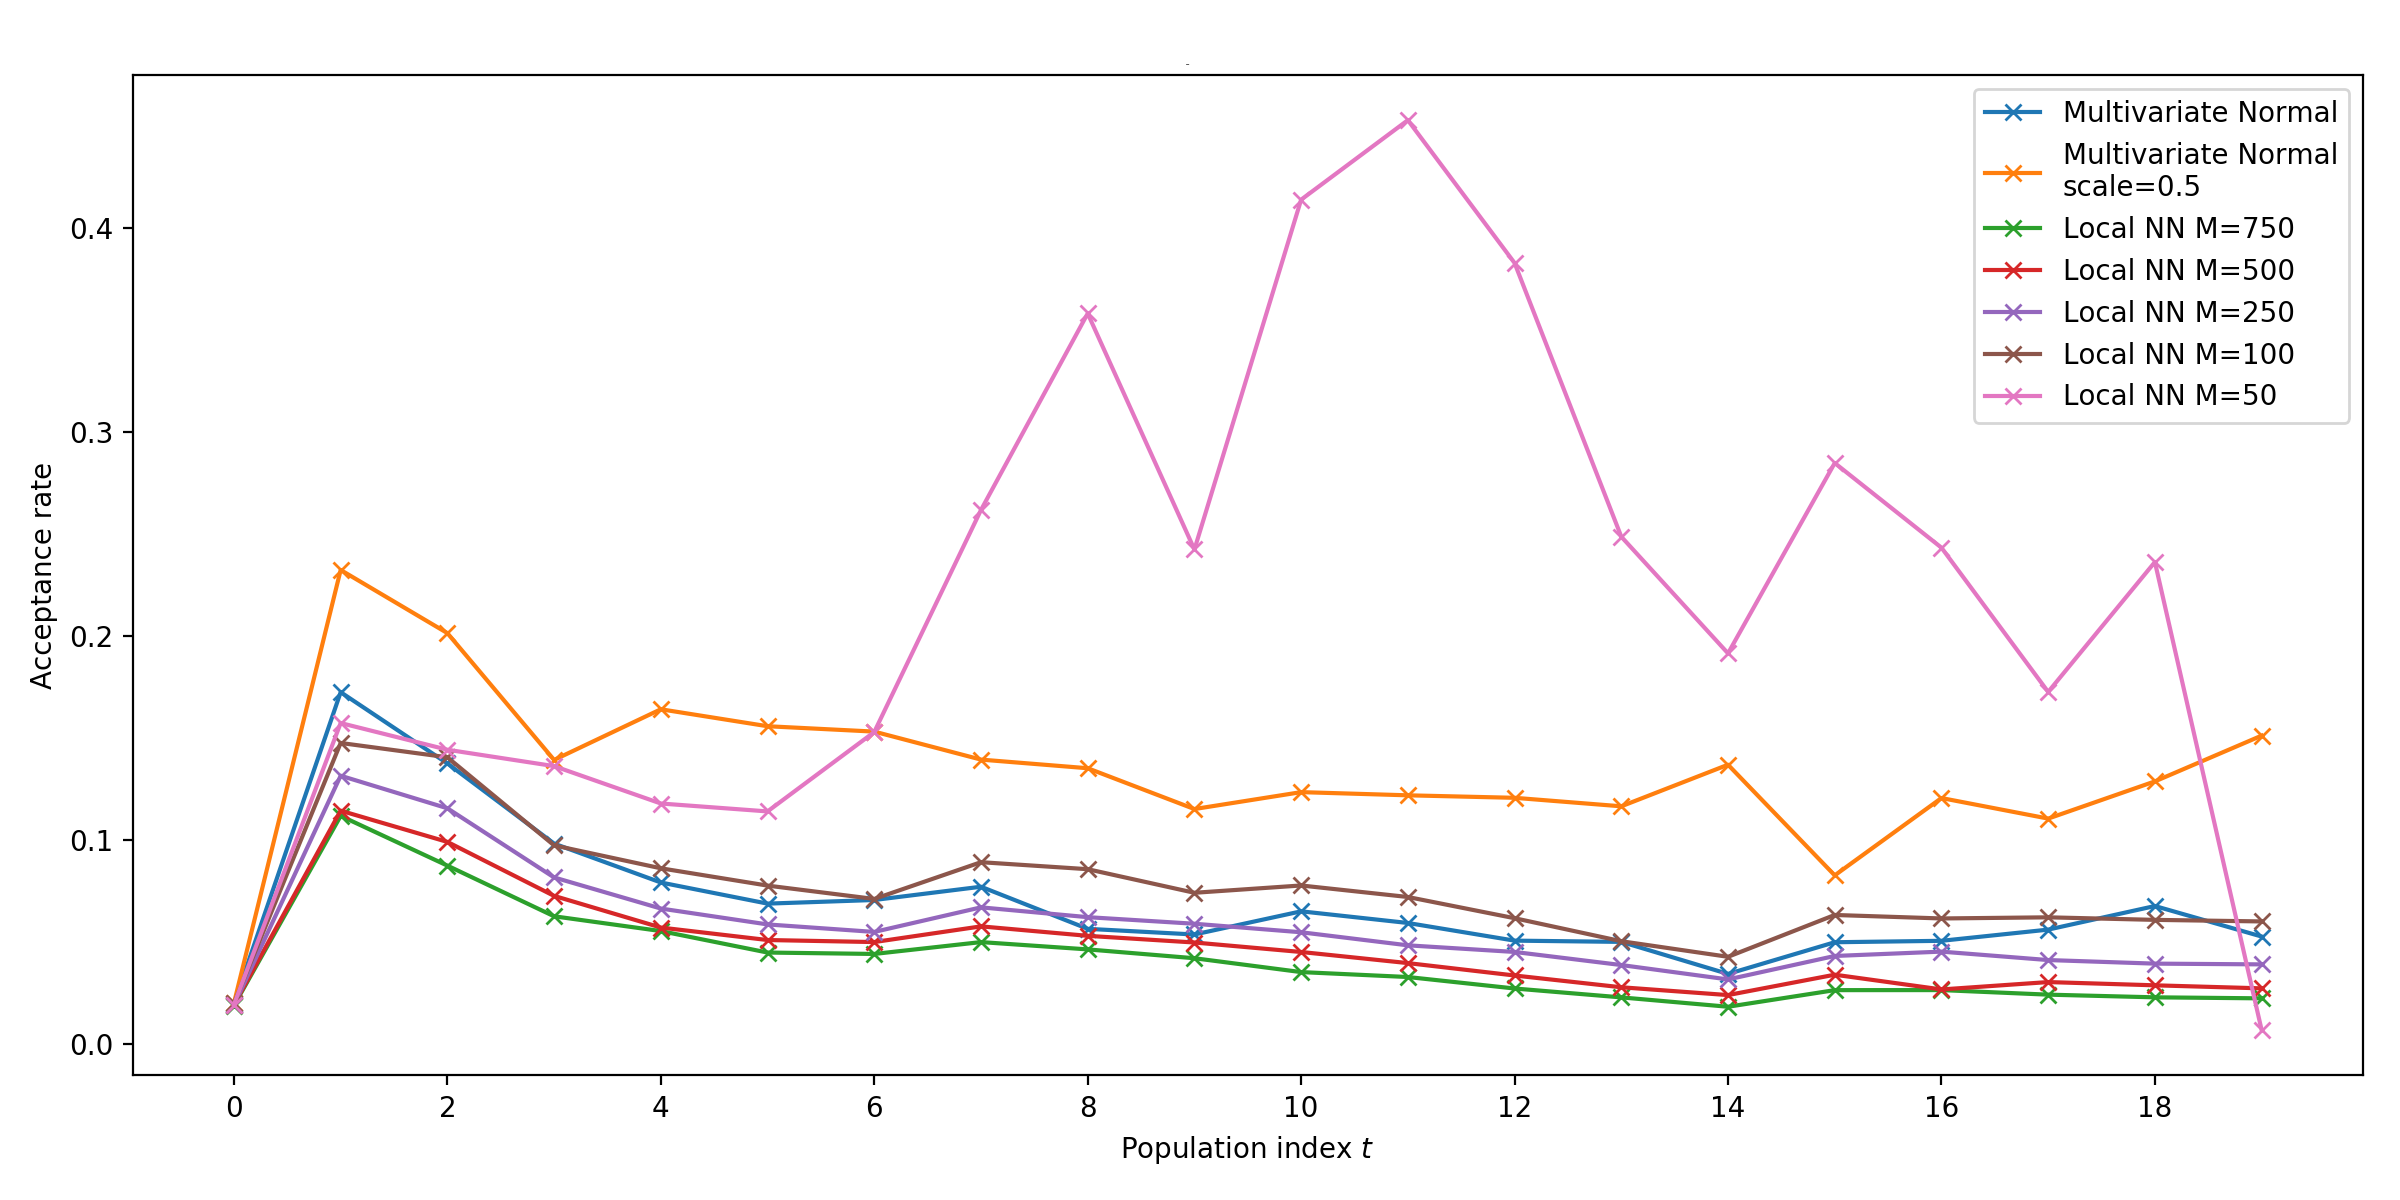
\includegraphics{fig/acceptance1.png}}
%     \end{center}
    
%     \caption{Acceptance rates of different kernels}
%     \label{fig:acceptance1}
    
% \end{figure}


\subsubsection{Adaptive functions and factors}

[how adaptive distance work]

SMC can be more adaptive by introducing adaptive distance function and adaptive population; besides, factors can be applied to manually `normalise' the data.

The trivial distance function is set to Euclidean distance (2-norm distance)

\begin{align}
    \label{eq:dis}
    D=\sqrt{\sum_i \Delta x_i^2}
\end{align}

where $i$ is the index of data points and $\Delta x_i$ is the discrepancy between  observed data and simulated data at data point $i$, i.e. $\Delta x_i = x_{i, simulated}-x_{i, observed}$. In this case data points are 12 time points of four variables i.e. 48 data points in total.

A weighted 2-norm distance can be written as 

\begin{align}
    \label{dis_w}
    D=\sqrt{\sum_i w_i \Delta x_i^2}
\end{align}

where a weight $w_i$ is assigned to every data point. If data point $i$ have a higher weight, then the data value is regeared to be more informative, i.e. giving more help in inferring the true posteriors; weights can be either pre-set according to prior knowledge of the problem, or using adaptive method to be dynamically calculated according to , known as adaptive distance. 

Adaptive distance is changing the weights of all data points after each generation iteration, trying to assign informative data points higher weights. Additionally, implementation of adaptive in \verb|pyABC| also introduces additional factors $f_i$ multiplied to weights \cite{ref:adpt_dis} 

\begin{align}
    \label{dis_w}
    D=\sqrt{\sum_i f_iw_i \Delta x_i^2}
\end{align}

Factor is helpful as an option for efficiency. When some data points are equally informative, the manually pre-defined can make the distance more focused on certain data point, or behave like a normalisation that can balance the scales of different summarised statistics (here is the 48 mean values). There are two appliance case studied: (1) factors used as an normalisation option ans (2) factors used to give more focus on some features of the observed data. For (2), as we noticed that the main features (e.g. rapid increase, peaks, fluctuations) are mostly observed in the first half of the time points i.e. 0 - 30 hpl, factors are tried in the later parameter estimation of real data where a more accurate fit of the curve is desired.

Adaptive population \cite{ref:adpt_pop} can adapt the population size of each generation according to the 

[what is factor]

[what is adaptive distance]

\subsubsection{Experiments results}

\paragraph{Conclusion}



\subsubsection{Data size, prior range, population size and generations}

[experiments plan]

\subsubsection{Experiments results}

\paragraph{Conclusion}





\subsection{Implementations and code}

[ABC implementations details, e.g. distance, population, ODE related functions]

[how the code is developed and built]

\section{Model comparison}

[comparison of model 1, 2 and 3]

[further comparison of model 3, 4 and 5]

\section{Performance experiments}

The performance experiments are designed to explore the parallel performance of ABC SMC implementations. Usually ABC SMC is a time-consuming and computation intensive task and usually is executed on large clusters. The scheduling strategy, implementation details and many other factors can affect the parallel efficiency.

[MORE meanings of the performance study]

\subsection{Scaling-up}

First experiments are designed to illustrate the scaling-up performance. The program used here is an implementation of ABc SMC on model 5. The details of the ABC SMC settings is listed below

\begin{itemize}
    \item Prior distribution: default to log-uniform distribution [$1\times 10^{-6}$, 50] for all the 12 parameters
    \item threshold schedule: median epsilon
    \item No factors, no adaptive distance or adaptive population applied
    \item Population size is 2000, with 20 generations
\end{itemize}

[HOW PYABC parallelise the sampling]

For HPC systems like Cirrus, \verb|pyabc| uses \verb|multiprocessing| for multi-core parallel sampling. By default if the number of cores is not specified, it will automatically read the number of available cores and use them all. Cirrus has a 36-core CPU which support hyperthreading, such that the maximal number of cores available to \verb|multiprocessing| is 72.

The program is executed on Cirrus, using 8, 12, 16, 24, 36, 54 and 72 cores respectively. Each run is repeated 5 times. The average execution time, required sampling numbers are recorded. Hyperthreading is enabled when using 54 and 72 cores. The access to the node that contains computation cores is exclusive, such that the execution would not be affected by other programs of operations.

The implementation of ABC SMC in \verb|pyabc| enables the parallelisation of sampling, which is the must time-consuming part. The rest part of the program is mostly not parallelised, e.g. database I/O and reductions operations. The sampling process involves sampling, perturbation and test of the acceptance criteria, all of which are computation-intensive. 

In practice, using ABC SMC to estimate the parameters of a given model could cost up to several hundred of hours if the computational resources is limited[REF]. The performance experiment result could provide a reference that illustrate that how the efficiency changes when scaling-up or the trade-offs in computational resources' cost and their benefit.

\subsection{Profiling}

The performance could also be analysed given a profiling report. The second experiment profiles the program to reveal the detailed time consumption for each operation and the possible bottleneck, according to which we could find the hot-spot of program and given possible suggestions on improving the performance. 

In this case, profile tools \verb|cProfile| and \verb|yappi| is used in PyCharm IDE.



\chapter{Results and Discussions}

[WHAT results is outputted and WHAT topics are discussed]

\section{ABC SMC results}

[inferred parameters: joint distribution, estimated values and simulated trajectory for each models; sensitivity; features of the inferred model]

[model selections result; bayes factor]

\section{Performance experiments}

[scaling-up performance: speed-up and efficiency]

[profiling results: hot-spot and possible improvements]

\section{Discussions}

[goodness of fit (evaluation); preferred models and effects of modification to basic model]

[efficiency and trade-offs in scaling-up]

[POSSIBLE: compare to exact inference; compared to other implementations]

[limitations]

\chapter{Future works}

[something not done as scheduled]

[interesting topics to look inside]

[moving to generalisations]

\chapter{Conclusions}

[what is studied]

[to what extend]

[how good is the result]

[summary of the findings and advise]

[thanks]

\appendix
% the appendix command just changes heading styles for appendices.

\chapter{System and software environment}

\section{ABC SMC implementation}

\section{Data analysis}

\chapter{Data and settings}




\section{Infer-back experiments}

\subsection{Parameter values used to generate synthetic data}

\begin{table}[h!]
    \centering
    \begin{tabular}{|c c c|} 
     \hline
     Parameter & Value & Unit\\ [0.5ex] 
     \hline\hline
     $\lambda_N$ & 2.1989 & $cell/h$  \\ 
     $\kappa_{N\beta}$ & 3.9627 & $cell/(unit\cdotp h)$\\
     $\mu_N$ & 1.7219 & $h^{-1}$\\
     $\nu_{N\Phi}$ & 0.2195 & $cell^{-1}\cdotp h^{-1}$ \\
     \hline
     $\lambda_\Phi$ & 1.3146 & $cell/h$ \\
     $\kappa_{\Phi\beta}$ & 0.1235 & $cell/(unit\cdotp h)$ \\
     $\mu_\Phi$ & 0.1454 & $h^{-1}$ \\
     \hline
     $s_{\beta N}$ & 6.5536 & $unit/(cell\cdotp h)$ \\
     $i_{\beta\Phi}$ & 1.7062 & $cell^{-1}$ \\
     $\mu_\beta$ & 0.5212 & $h^{-1}$ \\
     \hline
     $s_{\alpha\Phi}$ & 10.2416 & $unit/(cell\cdotp h)$ \\
     $\mu_\alpha$ & 19.6642 & $h^{-1}$ \\
    [1ex] 
     \hline
    \end{tabular}
    \caption{Parameter values}
    \label{table:m1}
\end{table}

\section{Kernel experiment: median epsilon schedule}

\begin{figure}

    \begin{center}
    \resizebox{1.0\hsize}{!}{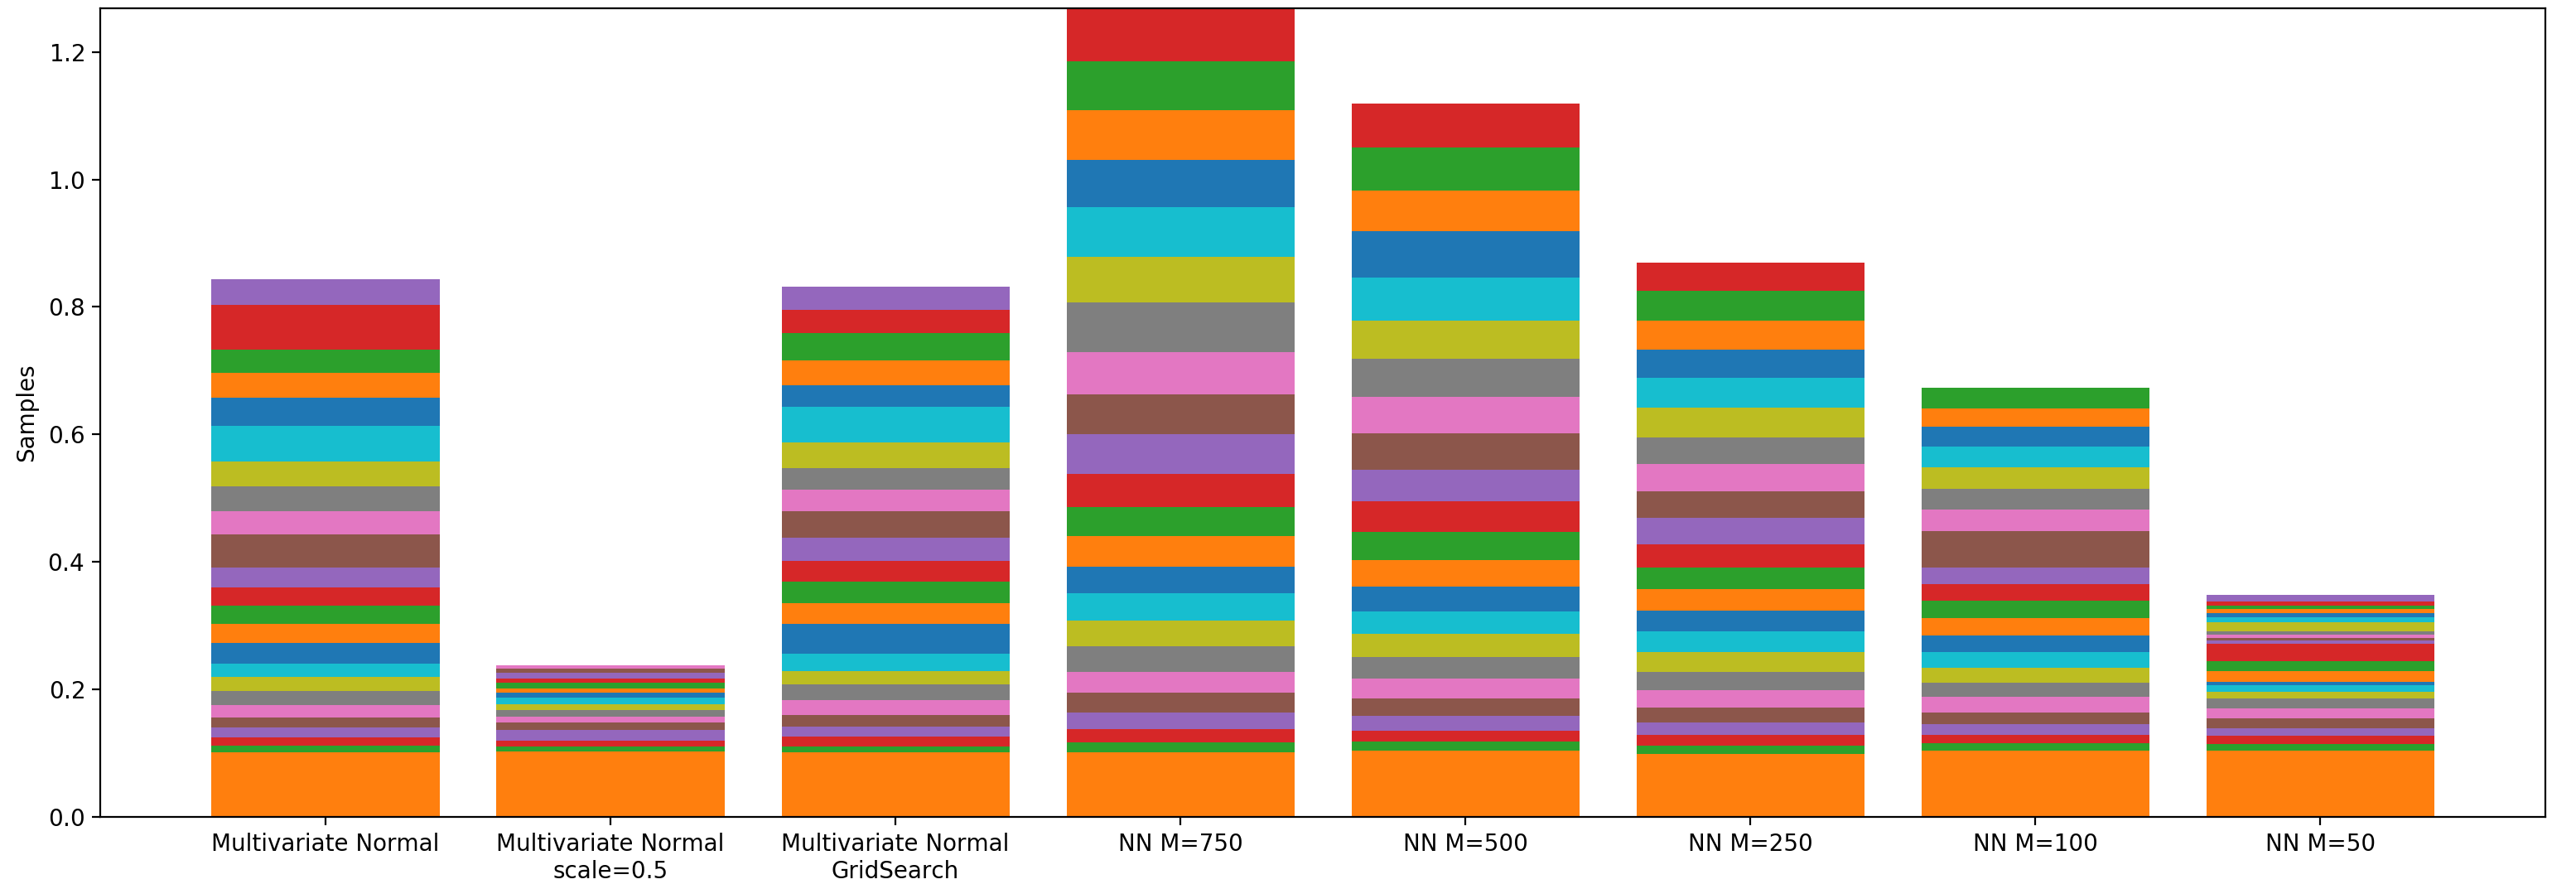
\includegraphics{fig/kernel2.png}}
    \end{center}
    
    \caption{Total sampling size} 
    \label{fig:kernel2}

    \begin{center}
        \resizebox{1.0\hsize}{!}{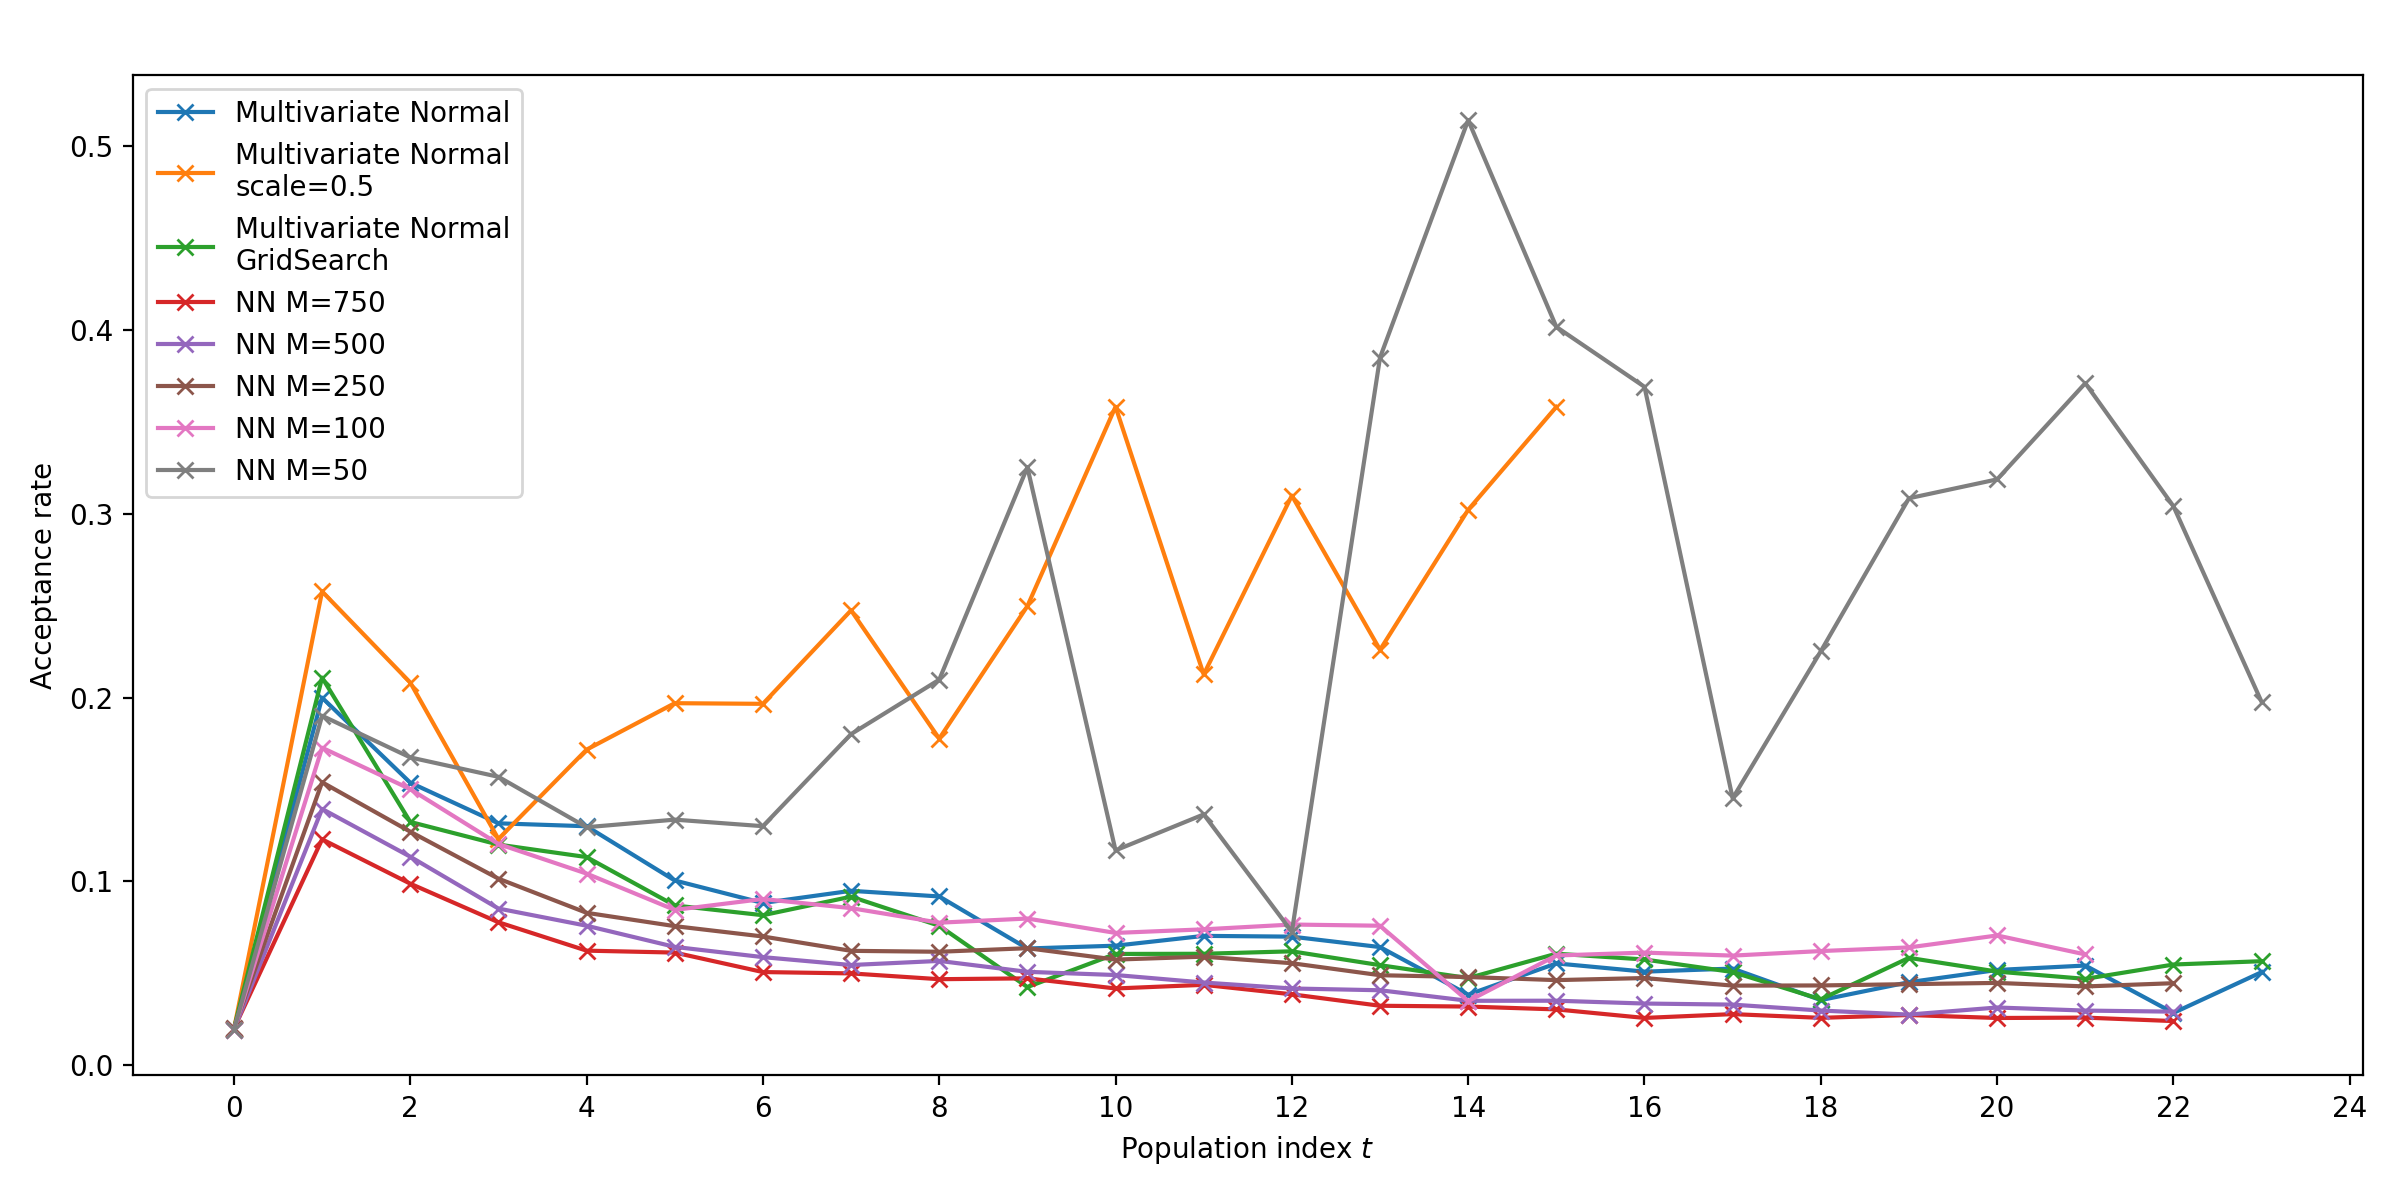
\includegraphics{fig/acceptance2.png}}
        \end{center}
        
        \caption{Acceptance rates} 
        \label{fig:acceptance2}
    
\end{figure}





\begin{thebibliography}{100}

\bibitem{ref:lam} L.Lamport. {\em 1986 Latex User's Guide
and Reference Manual.} Addison Wesley. pp242.

\bibitem{ref:bloggs} F.Bloggs. {\em 1993 Latex Users do it
in Environments} Int. Journal of Silly Findings. pp 23-29.

\bibitem{ref:Tsarouchas} Tsarouchas, T.M., Wehner, D., Cavone, L., Munir, T., Keatinge, M., Lambertus, M., Underhill, A., Barrett, T., Kassapis, E., Ogryzko, N. and Feng, Y., 2018. Dynamic control of proinflammatory cytokines Il-1$\beta$ and Tnf-$\alpha$ by macrophages in zebrafish spinal cord regeneration. Nature communications, 9(1), pp.1-17.

\bibitem{ref:pyabc} Klinger, E., Rickert, D. and Hasenauer, J., 2018. pyABC: distributed, likelihood-free inference. Bioinformatics, 34(20), pp.3591-3593.

\bibitem{ref:kernel} Filippi, S., Barnes, C. P., Cornebise, J., and Stumpf, M..H. (2013). On optimality of kernels for approximate Bayesian computation using sequential Monte Carlo. Statistical Applications in Genetics and Molecular Biology 12, 1, 87-107.

\bibitem{ref:abcsysbio} Liepe, J., Kirk, P., Filippi, S., Toni, T., Barnes, C.P., and Stumpf, M.P.H., 2014. A framework for parameter estimation and model selection from experimental data in systems biology using approximate Bayesian computation. Nature Protocols. 9 (2) pp. 439–456. 

\bibitem{ref:compare} Daly AC, Cooper J, GavaghanDJ, Holmes C. 2017. Comparing two sequentialMonte Carlo samplers for exact andapproximate Bayesian inference on biologicalmodels.J. R. Soc. Interface14: 20170340.

\bibitem{ref:disease} Minter, A. and Retkute, R., 2019. Approximate Bayesian Computation for infectious disease modelling. Epidemics, 29, p.100368.

\bibitem{ref:adpt_dis} Prangle, D., 2017. Adapting the ABC distance function. Bayesian Analysis, 12(1), pp.289-309.

\bibitem{ref:adpt_pop} Klinger, E. and Hasenauer, J., 2017, September. A scheme for adaptive selection of population sizes in approximate Bayesian computation-sequential Monte Carlo. In International Conference on Computational Methods in Systems Biology (pp. 128-144). Springer, Cham.

\end{thebibliography}


\end{document}

